\documentclass[a4paper, hidelinks, 11pt, fleqn]{article}
\usepackage{geometry}
\usepackage{wrapfig}
\usepackage{tikz}
\usetikzlibrary{decorations.pathreplacing}
\usetikzlibrary{calc}
\usepackage{listings}
\usepackage{color}
\usepackage{amsmath}
\usepackage{mathtools}
\geometry{letterpaper}
\usepackage{graphicx}
\usepackage{subcaption}
\usepackage{hyperref}
\usepackage{amssymb}

\definecolor{codegreen}{rgb}{0,0.6,0}
\definecolor{codegray}{rgb}{0.5,0.5,0.5}
\definecolor{lightgray}{rgb}{0.7,0.7,0.7}
\definecolor{codepurple}{rgb}{0.58,0,0.82}
\definecolor{backcolour}{rgb}{0.92,0.92,0.92}

\renewcommand{\lstlistingname}{Algorithm}% Listing -> Algorithm

\lstdefinestyle{mystyle}{
	backgroundcolor=\color{backcolour},   
	commentstyle=\color{codegray},
	keywordstyle=\color{red},
	numberstyle=\tiny\color{lightgray},
	stringstyle=\color{codepurple},
	basicstyle=\footnotesize,
	breakatwhitespace=false,         
	breaklines=true,                 
	captionpos=b,                    
	keepspaces=true,                 
	numbers=left,                    
	numbersep=5pt,                  
	showspaces=false,                
	showstringspaces=false,
	showtabs=false,                  
	tabsize=4
}

\lstset{style=mystyle}



%SetDrawFunctions

\newcommand{\hole}[3] % x in cm, y in cm, radius in mm
{ 
	% draw hole
	\draw (#1,#2) circle (#3mm);
	% crosshair
	\draw (#1,#2-0.05) -- (#1,#2+0.05);
	\draw (#1-0.05,#2) -- (#1+0.05,#2);
	% centering lines
	\draw (#1,#2-0.1*#3-0.05) -- (#1,#2-0.1);
	\draw (#1,#2+0.1) -- (#1,#2+0.1*#3+0.05);
	\draw (#1-0.1*#3-0.05,#2) -- (#1-0.1,#2);
	\draw (#1+0.1,#2) -- (#1+0.1*#3+0.05,#2);
}
\newcommand{\dimsv}[3] % start, end, x
{
	\draw (#3-0.2,#1) -- (#3+0.2,#1);
	\draw[<-] (#3,#1) -- (#3,{(#1+#2)/2-0.2});
	\draw (#3,{(#1+#2)/2}) node {\footnotesize \pgfmathparse{(#2 - #1)*10} \pgfmathprintnumber{\pgfmathresult} };
	\draw[->] (#3,{(#1+#2)/2+0.2}) -- (#3,#2);
	\draw (#3-0.2,#2) -- (#3+0.2,#2);
}
\newcommand{\dimsh}[3] % start, end, y
{
	\draw (#1,#3-0.1) -- (#1,#3+0.1);
	\draw[<-] (#1,#3) -- ({(#1+#2)/2-0.3},#3);
	\draw ({(#1+#2)/2},#3) node {\footnotesize \pgfmathparse{(#2 - #1)*10} \pgfmathprintnumber{\pgfmathresult} };
	\draw[->] ({(#1+#2)/2+0.3},#3) -- (#2,#3);
	\draw (#2,#3-0.1) -- (#2,#3+0.1);
}

%SetFonts
\newtagform{brackets}{[}{]}
\usetagform{brackets}

\title{\textbf{CNC Router}}
\author{Patrick Sorn}
\date{Version 2.0}

\begin{document}
\maketitle
\tableofcontents 
\pagebreak
\section{Introduction}
\pagebreak
\section{Portal}
\subsection{Spindle X mount}
\subsubsection{Base Plate}
\begin{figure}[ht!]
	\centering
	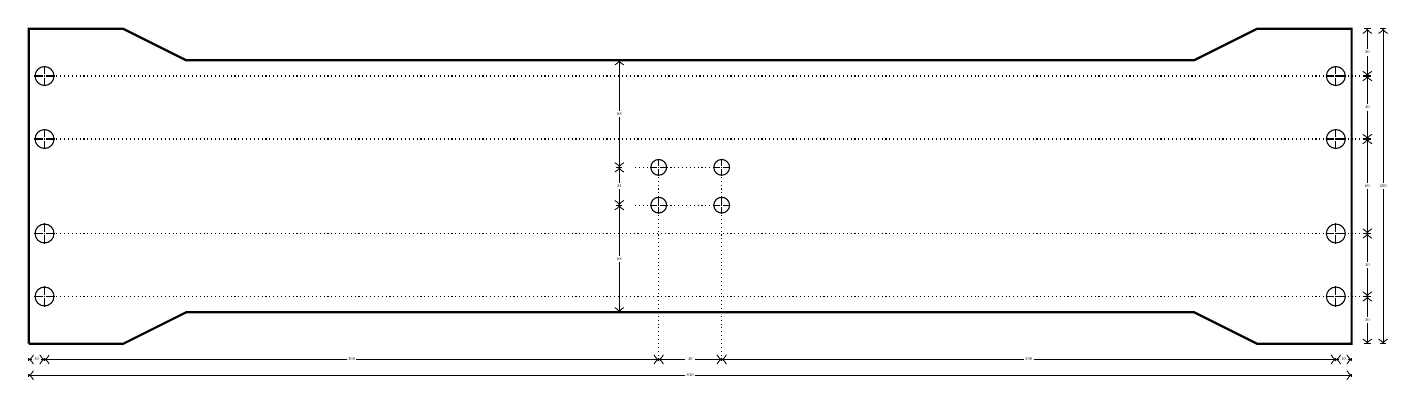
\begin{tikzpicture}[scale=0.2, every node/.style={scale=0.2}]
	% raw plate: 84cm x 20cm x 12mm
	% scale 1:5
	\draw[thick] (0, 0) -- (6, 0) -- (10, 2) -- (74, 2) -- (78, 0) -- (84, 0) -- (84, 20) -- (78, 20) -- (74, 18) -- (10, 18) -- (6, 20) -- (0, 20) -- (0, 0);
	\hole{1}{3}{6};
	\hole{1}{7}{6};
	\hole{1}{13}{6};
	\hole{1}{17}{6};
	
	\hole{83}{3}{6};
	\hole{83}{7}{6};
	\hole{83}{13}{6};
	\hole{83}{17}{6};
	
	\hole{40}{8.8}{5};
	\hole{40}{11.2}{5};
	\hole{44}{8.8}{5};
	\hole{44}{11.2}{5};
	
	\dimsh{0}{1}{-1};
	\dimsh{1}{40}{-1};
	\dimsh{40}{44}{-1};
	\dimsh{44}{83}{-1};
	\dimsh{83}{84}{-1};
	\dimsh{0}{84}{-2};
	
	\draw[densely dotted] (40, -1) -- (40, 8.3);
	\draw[densely dotted] (40, 9.3) -- (40, 10.7);
	\draw[densely dotted] (44, -1) -- (44, 8.3);
	\draw[densely dotted] (44, 9.3) -- (44, 10.7);
	
	\dimsv{0}{3}{85};
	\dimsv{3}{7}{85};
	\dimsv{7}{13}{85};
	\dimsv{13}{17}{85};
	\dimsv{17}{20}{85};
	\dimsv{0}{20}{86};
	
	%\draw[densely dotted] (-1, 3) -- (0.5, 3);
	\draw[densely dotted] (1.5, 3) -- (82.5, 3);
	\draw[densely dotted] (83.5, 3) -- (85, 3);
	%\draw[densely dotted] (-1, 7) -- (0.5, 7);
	\draw[densely dotted] (1.5, 7) -- (82.5, 7);
	\draw[densely dotted] (83.5, 7) -- (85, 7);
	%\draw[densely dotted] (-1, 13) -- (0.5, 13);
	\draw[densely dotted] (1.5, 13) -- (82.5, 13);
	\draw[densely dotted] (83.5, 13) -- (85, 13);
	%\draw[densely dotted] (-1, 17) -- (0.5, 17);
	\draw[densely dotted] (1.5, 17) -- (82.5, 17);
	\draw[densely dotted] (83.5, 17) -- (85, 17);
	
	\dimsv{2}{8.8}{37.5};
	\dimsv{8.8}{11.2}{37.5};
	\dimsv{11.2}{18}{37.5};
	
	\draw[densely dotted] (38.5, 8.8) -- (39.5, 8.8);
	\draw[densely dotted] (40.5, 8.8) -- (44.5, 8.8);
	\draw[densely dotted] (38.5, 11.2) -- (39.5, 11.2);
	\draw[densely dotted] (40.5, 11.2) -- (44.5, 11.2);

	\end{tikzpicture}
\caption{Base Plate.}
\label{fig:base_plate}
\end{figure}
\begin{figure}[ht!]
	\centering
	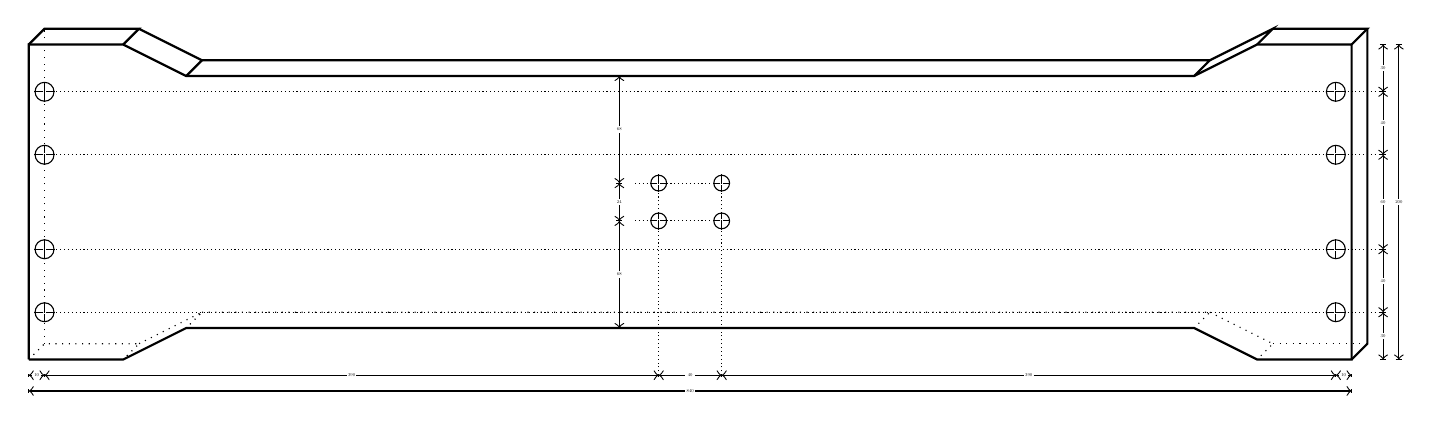
\begin{tikzpicture}[scale=0.2, every node/.style={scale=0.2}]
	% raw plate: 84cm x 20cm x 12mm
	% scale 1:5
	\draw[thick] (0, 0) -- (6, 0) -- (10, 2) -- (74, 2) -- (78, 0) -- (84, 0) -- (84, 20) -- (78, 20) -- (74, 18) -- (10, 18) -- (6, 20) -- (0, 20) -- (0, 0);
	\draw[thick] (0, 20) -- (1, 21) -- (7, 21) -- (6, 20);
	\draw[thick] (7, 21) -- (11, 19) -- (10, 18);
	\draw[thick] (11, 19) -- (75, 19) -- (74, 18);
	\draw[thick] (75, 19) -- (79, 21) -- (78, 20);
	\draw[thick] (79, 21) -- (85, 21) -- (84, 20);
	\draw[thick] (85, 21) -- (85, 1) -- (84, 0);
	\draw[dotted] (0, 0) -- (1, 1) -- (7, 1) -- (6, 0);
	\draw[dotted] (7, 1) -- (11, 3) -- (10, 2);
	\draw[dotted] (11, 3) -- (75, 3) -- (74, 2);
	\draw[dotted] (75, 3) -- (79, 1) -- (78, 0);
	\draw[dotted] (79, 1) -- (85, 1);
	\draw[dotted] (1, 1) -- (1, 21);
	\hole{1}{3}{6};
	\hole{1}{7}{6};
	\hole{1}{13}{6};
	\hole{1}{17}{6};
	
	\hole{83}{3}{6};
	\hole{83}{7}{6};
	\hole{83}{13}{6};
	\hole{83}{17}{6};
	
	\hole{40}{8.8}{5};
	\hole{40}{11.2}{5};
	\hole{44}{8.8}{5};
	\hole{44}{11.2}{5};
	
	\dimsh{0}{1}{-1};
	\dimsh{1}{40}{-1};
	\dimsh{40}{44}{-1};
	\dimsh{44}{83}{-1};
	\dimsh{83}{84}{-1};
	\dimsh{0}{84}{-2};
	
	\draw[densely dotted] (40, -1) -- (40, 8.3);
	\draw[densely dotted] (40, 9.3) -- (40, 10.7);
	\draw[densely dotted] (44, -1) -- (44, 8.3);
	\draw[densely dotted] (44, 9.3) -- (44, 10.7);
	
	\dimsv{0}{3}{86};
	\dimsv{3}{7}{86};
	\dimsv{7}{13}{86};
	\dimsv{13}{17}{86};
	\dimsv{17}{20}{86};
	\dimsv{0}{20}{87};
	
	%\draw[densely dotted] (-1, 3) -- (0.5, 3);
	\draw[densely dotted] (1.5, 3) -- (82.5, 3);
	\draw[densely dotted] (83.5, 3) -- (86, 3);
	%\draw[densely dotted] (-1, 7) -- (0.5, 7);
	\draw[densely dotted] (1.5, 7) -- (82.5, 7);
	\draw[densely dotted] (83.5, 7) -- (86, 7);
	%\draw[densely dotted] (-1, 13) -- (0.5, 13);
	\draw[densely dotted] (1.5, 13) -- (82.5, 13);
	\draw[densely dotted] (83.5, 13) -- (86, 13);
	%\draw[densely dotted] (-1, 17) -- (0.5, 17);
	\draw[densely dotted] (1.5, 17) -- (82.5, 17);
	\draw[densely dotted] (83.5, 17) -- (86, 17);
	
	\dimsv{2}{8.8}{37.5};
	\dimsv{8.8}{11.2}{37.5};
	\dimsv{11.2}{18}{37.5};
	
	\draw[densely dotted] (38.5, 8.8) -- (39.5, 8.8);
	\draw[densely dotted] (40.5, 8.8) -- (44.5, 8.8);
	\draw[densely dotted] (38.5, 11.2) -- (39.5, 11.2);
	\draw[densely dotted] (40.5, 11.2) -- (44.5, 11.2);
	
	\end{tikzpicture}
	\caption{Base Plate 3D.}
	\label{fig:base_plate_3d}
\end{figure}
\newpage
\subsubsection{Front Plate}
\begin{figure}[ht!]
	\centering
	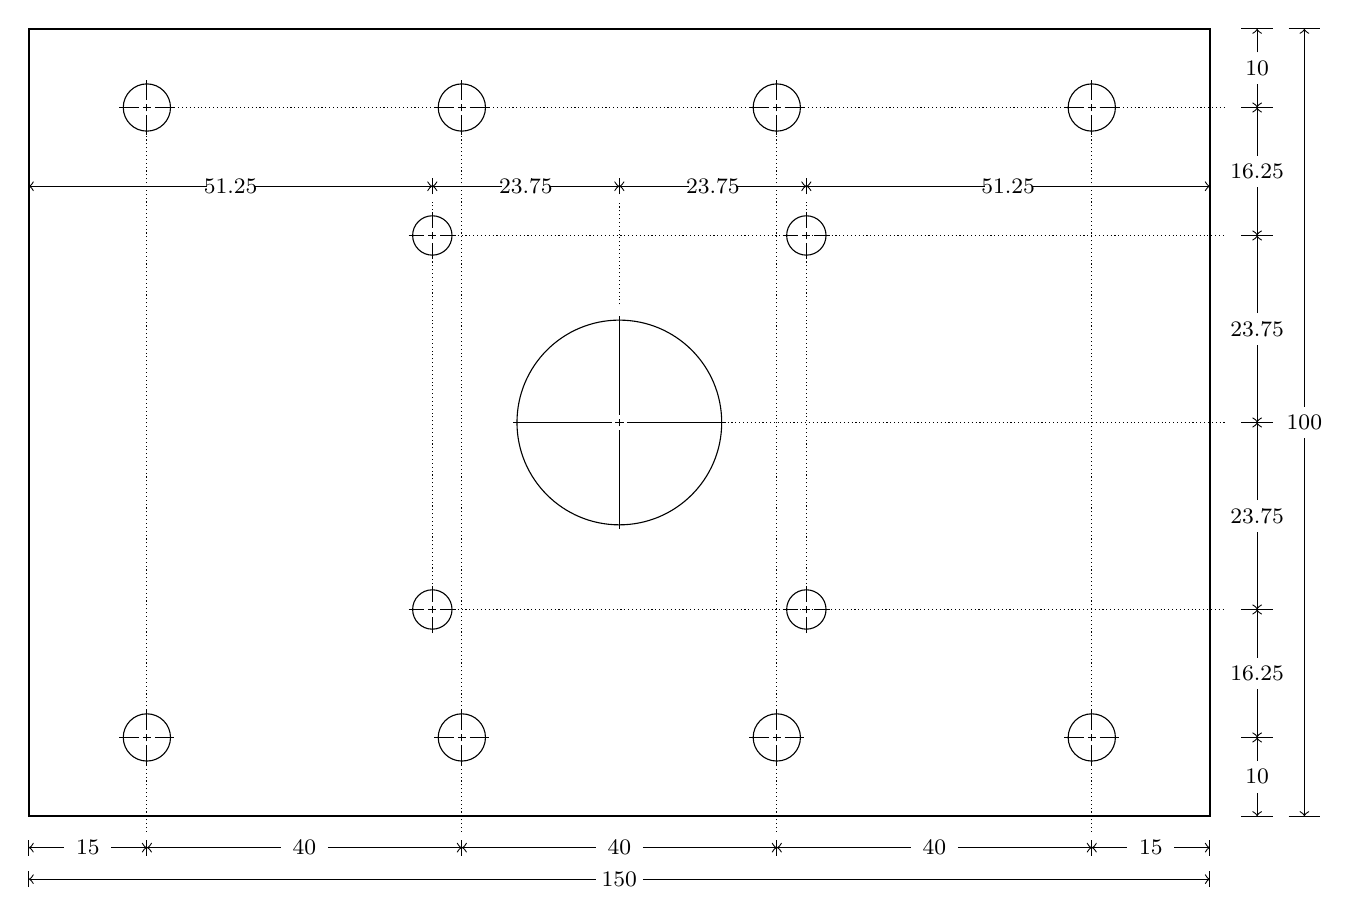
\begin{tikzpicture}
	% raw plate: 15cm x 9cm x 12mm
	% scale 1:5
	\draw[thick] (0, 0) rectangle (15, 10);
	%\draw[thick] (0, 10) -- (15, 10) -- (15, 7) -- (11, 0) -- (4, 0) -- (0, 7) -- (0, 10);
	\draw[dotted] (0, 6) -- (0, 0) -- (4, 0);
	\draw[dotted] (11, 0) -- (15, 0) -- (15, 7);
	\hole{1.5}{9}{3};
	\hole{5.5}{9}{3};
	\hole{9.5}{9}{3};
	\hole{13.5}{9}{3};
	
	\hole{1.5}{1}{3};
	\hole{5.5}{1}{3};
	\hole{9.5}{1}{3};
	\hole{13.5}{1}{3};
	
	\hole{7.5}{5}{13};
	
	\hole{5.125}{2.625}{2.5};
	\hole{5.125}{7.375}{2.5};
	\hole{9.875}{2.625}{2.5};
	\hole{9.875}{7.375}{2.5};
	
	\dimsh{0}{1.5}{-0.4};
	\dimsh{1.5}{5.5}{-0.4};
	\dimsh{5.5}{9.5}{-0.4};
	\dimsh{9.5}{13.5}{-0.4};
	\dimsh{13.5}{15}{-0.4};
	\dimsh{0}{15}{-0.8};
	
	\draw[densely dotted] (1.5, -0.2) -- (1.5, 0.8);
	\draw[densely dotted] (1.5, 1.2) -- (1.5, 8.8);
	\draw[densely dotted] (5.5, -0.2) -- (5.5, 0.8);
	\draw[densely dotted] (5.5, 1.2) -- (5.5, 8.8);
	\draw[densely dotted] (9.5, -0.2) -- (9.5, 0.8);
	\draw[densely dotted] (9.5, 1.2) -- (9.5, 8.8);
	\draw[densely dotted] (13.5, -0.2) -- (13.5, 0.8);
	\draw[densely dotted] (13.5, 1.2) -- (13.5, 8.8);
	
	\dimsh{0}{5.125}{8};
	\dimsh{5.125}{7.5}{8};
	\dimsh{7.5}{9.875}{8};
	\dimsh{9.875}{15}{8};
	
	\draw[densely dotted] (5.125, 7.5) -- (5.125, 7.8);
	\draw[densely dotted] (5.125, 2.8) -- (5.125, 7.1);
	\draw[densely dotted] (7.5, 6.5) -- (7.5, 7.8);
	\draw[densely dotted] (9.875, 7.5) -- (9.875, 7.8);
	\draw[densely dotted] (9.875, 2.8) -- (9.875, 7.1);
	
	\dimsv{0}{1}{15.6};
	\dimsv{1}{2.625}{15.6};
	\dimsv{2.625}{5}{15.6};
	\dimsv{5}{7.375}{15.6};
	\dimsv{7.375}{9}{15.6};
	\dimsv{9}{10}{15.6};
	\dimsv{0}{10}{16.2};
	
	%\draw[densely dotted] (-0.1, 2.625) -- (5, 2.625);
	\draw[densely dotted] (5.3, 2.625) -- (9.6, 2.625);
	\draw[densely dotted] (9.6, 2.625) -- (15.2, 2.625);
	%\draw[densely dotted] (-0.1, 5) -- (7, 5);
	\draw[densely dotted] (7.3, 5) -- (15.2, 5);
	%\draw[densely dotted] (-0.1, 7.375) -- (5, 7.375);
	\draw[densely dotted] (5.3, 7.375) -- (9.6, 7.375);
	\draw[densely dotted] (9.9, 7.375) -- (15.2, 7.375);
	
	%\draw[densely dotted] (-0.1, 9) -- (1.3, 9);
	\draw[densely dotted] (1.7, 9) -- (5.3, 9);
	\draw[densely dotted] (5.7, 9) -- (9.3, 9);
	\draw[densely dotted] (9.7, 9) -- (13.3, 9);
	\draw[densely dotted] (13.6, 9) -- (15.2, 9);
	
	
	\end{tikzpicture}
	\caption{Front Plate.}
	\label{fig:front_plate}
\end{figure}
\begin{figure}[ht!]
	\centering
	\begin{tikzpicture}
	% raw plate: 15cm x 9cm x 12mm
	% scale 1:5
	\draw[thick] (0, 0) rectangle (15, 10);
	\draw[thick] (0, 10) -- (1, 11) -- (16, 11) -- (15, 10);
	\draw[thick] (16, 11) -- (16, 1) -- (15, 0);
	\draw[dotted] (0, 0) -- (1, 1) -- (1, 11);
	%\draw[dotted] (1, 7) -- (16, 7);
	\draw[dotted] (1, 1) -- (16, 1);
	%\draw[dotted] (5, 1) -- (12, 1);
	
	\hole{1.5}{9}{3};
	\hole{5.5}{9}{3};
	\hole{9.5}{9}{3};
	\hole{13.5}{9}{3};
	
	\hole{1.5}{1}{3};
	\hole{5.5}{1}{3};
	\hole{9.5}{1}{3};
	\hole{13.5}{1}{3};
	
	\hole{7.5}{5}{13};
	
	\hole{5.125}{2.625}{2.5};
	\hole{5.125}{7.375}{2.5};
	\hole{9.875}{2.625}{2.5};
	\hole{9.875}{7.375}{2.5};
	
	\end{tikzpicture}
	\caption{Front Plate 3D.}
	\label{fig:front_plate_3d}
\end{figure}
\subsection{Spindle Y mount}
\subsubsection{Side Plate}
\begin{figure}[ht!]
	\centering
	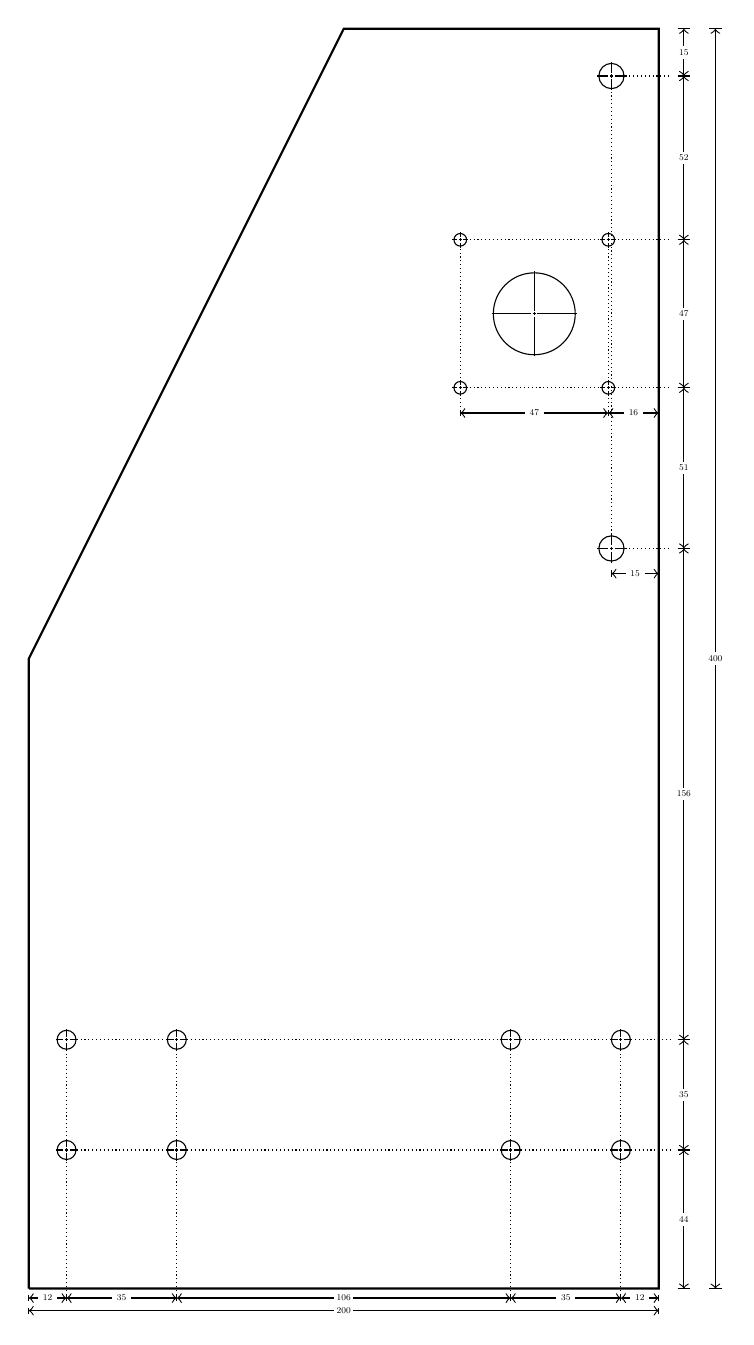
\begin{tikzpicture}[scale=0.4, every node/.style={scale=0.4}]
	% raw plate: 20cm x 40cm x 20mm
	% scale 2:5
	%\draw[thick] (0, 0) rectangle (10, 20);
	\draw[thick] (0, 0) -- (20, 0) -- (20, 40) -- (10, 40) -- (0, 20) -- (0, 0);
	%\draw[dotted] (0, 20) -- (0, 40) -- (10, 40);
	\hole{1.2}{4.4}{3};
	\hole{1.2}{7.9}{3};
	\hole{4.7}{4.4}{3};
	\hole{4.7}{7.9}{3};
	
	\hole{15.3}{4.4}{3};
	\hole{15.3}{7.9}{3};
	\hole{18.8}{4.4}{3};
	\hole{18.8}{7.9}{3};
	
	\hole{18.5}{23.5}{4};
	\hole{18.5}{38.5}{4};
	
	\hole{13.7}{28.6}{2};
	\hole{13.7}{33.3}{2};
	\hole{18.4}{28.6}{2};
	\hole{18.4}{33.3}{2};
	
	\hole{16.05}{30.95}{13};
	
	
	\dimsh{0}{1.2}{-0.3};
	\dimsh{1.2}{4.7}{-0.3};
	\dimsh{4.7}{15.3}{-0.3};
	\dimsh{15.3}{18.8}{-0.3};
	\dimsh{18.8}{20}{-0.3};
	\dimsh{0}{20}{-0.7};
	
	\draw[densely dotted] (1.2, -0.2) -- (1.2, 4.2);
	\draw[densely dotted] (1.2, 4.6) -- (1.2, 7.7);
	\draw[densely dotted] (4.7, -0.2) -- (4.7, 4.2);
	\draw[densely dotted] (4.7, 4.6) -- (4.7, 7.7);
	\draw[densely dotted] (15.3, -0.2) -- (15.3, 4.2);
	\draw[densely dotted] (15.3, 4.6) -- (15.3, 7.7);
	\draw[densely dotted] (18.8, -0.2) -- (18.8, 4.2);
	\draw[densely dotted] (18.8, 4.6) -- (18.8, 7.7);
	
	\dimsv{0}{4.4}{20.8};
	\dimsv{4.4}{7.9}{20.8};
	\dimsv{7.9}{23.5}{20.8};
	\dimsv{23.5}{28.6}{20.8};
	\dimsv{28.6}{33.3}{20.8};
	\dimsv{33.3}{38.5}{20.8};
	\dimsv{38.5}{40}{20.8};
	\dimsv{0}{40}{21.8};
	
	\draw[densely dotted] (1.4, 4.4) -- (4.5, 4.4);
	\draw[densely dotted] (4.9, 4.4) -- (15.1, 4.4);
	\draw[densely dotted] (15.5, 4.4) -- (18.6, 4.4);
	\draw[densely dotted] (19, 4.4) -- (20.4, 4.4);
	\draw[densely dotted] (1.4, 7.9) -- (4.5, 7.9);
	\draw[densely dotted] (4.9, 7.9) -- (15.1, 7.9);
	\draw[densely dotted] (15.5, 7.9) -- (18.6, 7.9);
	\draw[densely dotted] (19, 7.9) -- (20.4, 7.9);
	
	\draw[densely dotted] (18.7, 23.5) -- (20.4, 23.5);
	\draw[densely dotted] (18.7, 38.5) -- (20.4, 38.5);
	
	%\dimsh{0}{18.5}{22.7};
	\dimsh{18.5}{20}{22.7};
	
	\draw[densely dotted] (18.5, 23.7) -- (18.5, 38.3);
	
	\draw[densely dotted] (14, 28.6) -- (18.3, 28.6);
	\draw[densely dotted] (18.7, 28.6) -- (20.4, 28.6);
	\draw[densely dotted] (14, 33.3) -- (18.3, 33.3);
	\draw[densely dotted] (18.7, 33.3) -- (20.4, 33.3);
	
	%\dimsh{0}{13.7}{27.8};
	\dimsh{13.7}{18.4}{27.8};
	\dimsh{18.4}{20}{27.8};
	
	\draw[densely dotted] (13.7, 28) -- (13.7, 28.4);
	\draw[densely dotted] (13.7, 28.8) -- (13.7, 33.1);
	\draw[densely dotted] (18.4, 28) -- (18.4, 28.4);
	\draw[densely dotted] (18.4, 28.8) -- (18.4, 33.1);
	
	
	
	\end{tikzpicture}
\caption{Side Plate.}
\label{fig:side_plate}
\end{figure}
\newpage
\begin{figure}[ht!]
	\centering
	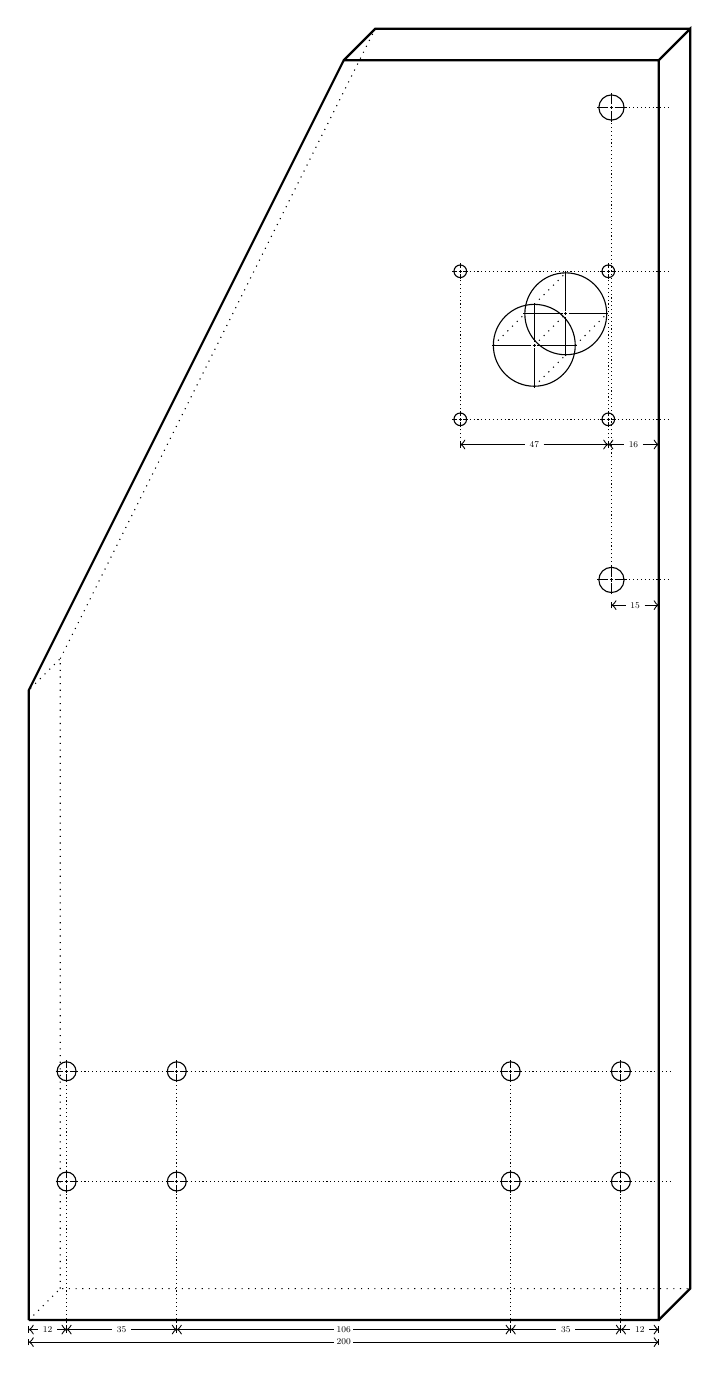
\begin{tikzpicture}[scale=0.4, every node/.style={scale=0.4}]
	% raw plate: 20cm x 40cm x 20mm
	% scale 2:5
	%\draw[thick] (0, 0) rectangle (10, 20);
	\draw[thick] (0, 0) -- (20, 0) -- (20, 40) -- (10, 40) -- (0, 20) -- (0, 0);
	\draw[thick] (20, 0) -- (21, 1) -- (21, 41)-- (20, 40);
	\draw[thick] (10, 40) -- (11, 41) -- (21, 41);
	\draw[dotted] (0, 0) -- (1, 1) -- (21, 1);
	\draw[dotted] (1, 1) -- (1, 21) -- (0, 20);
	\draw[dotted] (1, 21) -- (11, 41);
	%\draw[dotted] (0, 20) -- (0, 40) -- (10, 40);
	\hole{1.2}{4.4}{3};
	\hole{1.2}{7.9}{3};
	\hole{4.7}{4.4}{3};
	\hole{4.7}{7.9}{3};
	
	\hole{15.3}{4.4}{3};
	\hole{15.3}{7.9}{3};
	\hole{18.8}{4.4}{3};
	\hole{18.8}{7.9}{3};
	
	\hole{18.5}{23.5}{4};
	\hole{18.5}{38.5}{4};
	
	\hole{13.7}{28.6}{2};
	\hole{13.7}{33.3}{2};
	\hole{18.4}{28.6}{2};
	\hole{18.4}{33.3}{2};
	
	\hole{16.05}{30.95}{13};
	\hole{17.05}{31.95}{13};
	\draw[dotted] (16.05, 30.95) -- (17.05, 31.95);
	\draw[dotted] (14.75, 30.95) -- (15.75, 31.95);
	\draw[dotted] (17.35, 30.95) -- (18.35, 31.95);
	\draw[dotted] (16.05, 29.65) -- (17.05, 30.65);
	\draw[dotted] (16.05, 32.25) -- (17.05, 33.25);
	
	
	\dimsh{0}{1.2}{-0.3};
	\dimsh{1.2}{4.7}{-0.3};
	\dimsh{4.7}{15.3}{-0.3};
	\dimsh{15.3}{18.8}{-0.3};
	\dimsh{18.8}{20}{-0.3};
	\dimsh{0}{20}{-0.7};
	
	\draw[densely dotted] (1.2, -0.2) -- (1.2, 4.2);
	\draw[densely dotted] (1.2, 4.6) -- (1.2, 7.7);
	\draw[densely dotted] (4.7, -0.2) -- (4.7, 4.2);
	\draw[densely dotted] (4.7, 4.6) -- (4.7, 7.7);
	\draw[densely dotted] (15.3, -0.2) -- (15.3, 4.2);
	\draw[densely dotted] (15.3, 4.6) -- (15.3, 7.7);
	\draw[densely dotted] (18.8, -0.2) -- (18.8, 4.2);
	\draw[densely dotted] (18.8, 4.6) -- (18.8, 7.7);
	
	%\dimsv{0}{4.4}{20.8};
	%\dimsv{4.4}{7.9}{20.8};
	%\dimsv{7.9}{23.5}{20.8};
	%\dimsv{23.5}{28.6}{20.8};
	%\dimsv{28.6}{33.3}{20.8};
	%\dimsv{33.3}{38.5}{20.8};
	%\dimsv{38.5}{40}{20.8};
	%\dimsv{0}{40}{21.8};
	
	\draw[densely dotted] (1.4, 4.4) -- (4.5, 4.4);
	\draw[densely dotted] (4.9, 4.4) -- (15.1, 4.4);
	\draw[densely dotted] (15.5, 4.4) -- (18.6, 4.4);
	\draw[densely dotted] (19, 4.4) -- (20.4, 4.4);
	\draw[densely dotted] (1.4, 7.9) -- (4.5, 7.9);
	\draw[densely dotted] (4.9, 7.9) -- (15.1, 7.9);
	\draw[densely dotted] (15.5, 7.9) -- (18.6, 7.9);
	\draw[densely dotted] (19, 7.9) -- (20.4, 7.9);
	
	\draw[densely dotted] (18.7, 23.5) -- (20.4, 23.5);
	\draw[densely dotted] (18.7, 38.5) -- (20.4, 38.5);
	
	%\dimsh{0}{18.5}{22.7};
	\dimsh{18.5}{20}{22.7};
	
	\draw[densely dotted] (18.5, 23.7) -- (18.5, 38.3);
	
	\draw[densely dotted] (14, 28.6) -- (18.3, 28.6);
	\draw[densely dotted] (18.7, 28.6) -- (20.4, 28.6);
	\draw[densely dotted] (14, 33.3) -- (18.3, 33.3);
	\draw[densely dotted] (18.7, 33.3) -- (20.4, 33.3);
	
	%\dimsh{0}{13.7}{27.8};
	\dimsh{13.7}{18.4}{27.8};
	\dimsh{18.4}{20}{27.8};
	
	\draw[densely dotted] (13.7, 28) -- (13.7, 28.4);
	\draw[densely dotted] (13.7, 28.8) -- (13.7, 33.1);
	\draw[densely dotted] (18.4, 28) -- (18.4, 28.4);
	\draw[densely dotted] (18.4, 28.8) -- (18.4, 33.1);
	
	
	
	\end{tikzpicture}
	\caption{Side Plate 3D.}
	\label{fig:side_plate_3d}
\end{figure}
\newpage
\subsubsection{Rear Plate}
\begin{figure}[ht!]
	\centering
	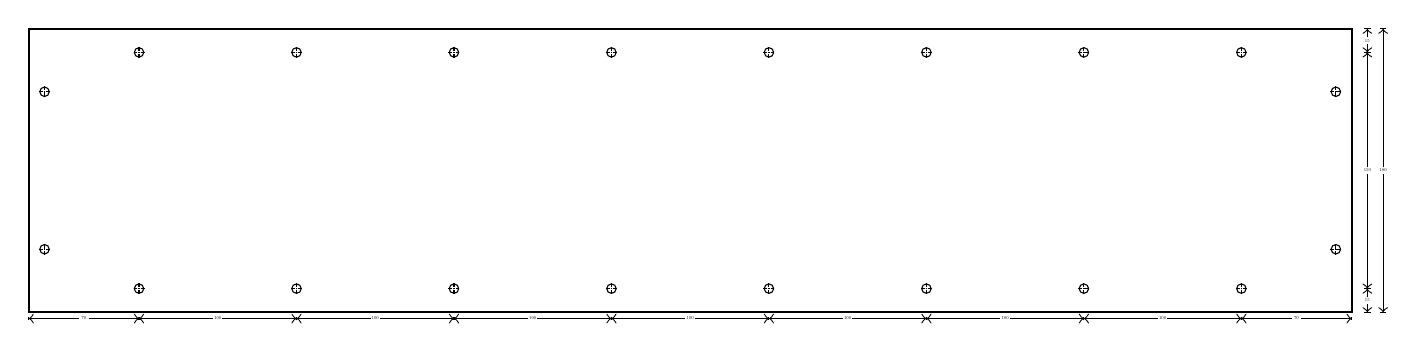
\begin{tikzpicture}[scale=0.2, every node/.style={scale=0.2}]
	% raw plate: 84cm x 18cm x 10mm
	% scale 1:5
	\draw[thick] (0, 0) rectangle (84, 18);
	\hole{1}{4}{3};
	\hole{1}{14}{3};
	\hole{83}{4}{3};
	\hole{83}{14}{3};
	
	\hole{7}{1.5}{3};
	\hole{7}{16.5}{3};
	\hole{17}{1.5}{3};
	\hole{17}{16.5}{3};
	\hole{27}{1.5}{3};
	\hole{27}{16.5}{3};
	\hole{37}{1.5}{3};
	\hole{37}{16.5}{3};
	\hole{47}{1.5}{3};
	\hole{47}{16.5}{3};
	\hole{57}{1.5}{3};
	\hole{57}{16.5}{3};
	\hole{67}{1.5}{3};
	\hole{67}{16.5}{3};
	\hole{77}{1.5}{3};
	\hole{77}{16.5}{3};
	
	\dimsh{0}{7}{-0.4};
	\dimsh{7}{17}{-0.4};
	\dimsh{17}{27}{-0.4};
	\dimsh{27}{37}{-0.4};
	\dimsh{37}{47}{-0.4};
	\dimsh{47}{57}{-0.4};
	\dimsh{57}{67}{-0.4};
	\dimsh{67}{77}{-0.4};
	\dimsh{77}{84}{-0.4};
	
	\dimsv{0}{1.5}{85};
	\dimsv{1.5}{16.5}{85};
	\dimsv{16.5}{18}{85};
	\dimsv{0}{18}{86};
	\end{tikzpicture}
\caption{Rear Plate.}
\label{fig:rear_plate}
\end{figure}
\begin{figure}[ht!]
	\centering
	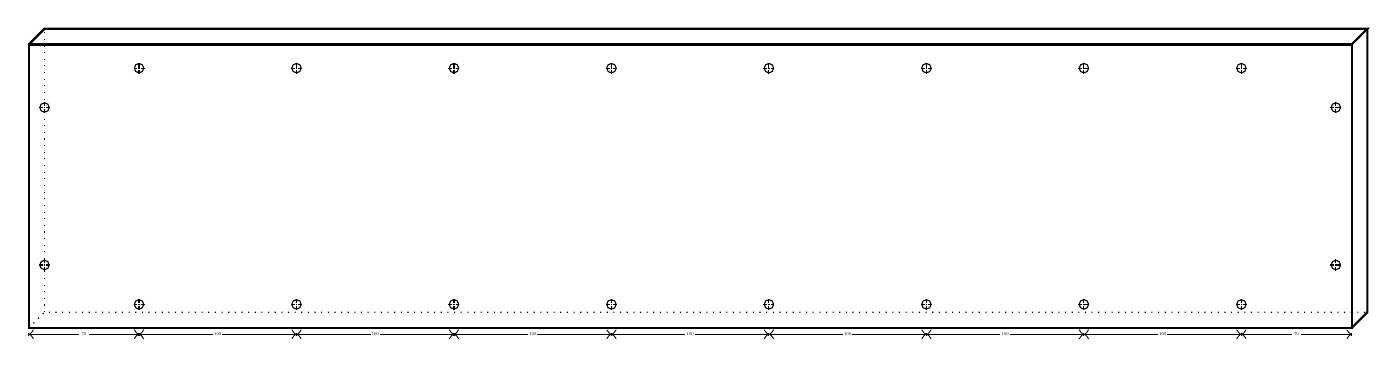
\begin{tikzpicture}[scale=0.2, every node/.style={scale=0.2}]
	% raw plate: 84cm x 18cm x 10mm
	% scale 1:5
	\draw[thick] (0, 0) rectangle (84, 18);
	\draw[thick] (0, 18) -- (1, 19) -- (85, 19) -- (84, 18);
	\draw[thick] (85, 19) -- (85, 1) -- (84, 0);
	\draw[dotted] (0, 0) -- (1, 1) -- (85, 1);
	\draw[dotted] (1, 1) -- (1, 19);
	\hole{1}{4}{3};
	\hole{1}{14}{3};
	\hole{83}{4}{3};
	\hole{83}{14}{3};
	
	\hole{7}{1.5}{3};
	\hole{7}{16.5}{3};
	\hole{17}{1.5}{3};
	\hole{17}{16.5}{3};
	\hole{27}{1.5}{3};
	\hole{27}{16.5}{3};
	\hole{37}{1.5}{3};
	\hole{37}{16.5}{3};
	\hole{47}{1.5}{3};
	\hole{47}{16.5}{3};
	\hole{57}{1.5}{3};
	\hole{57}{16.5}{3};
	\hole{67}{1.5}{3};
	\hole{67}{16.5}{3};
	\hole{77}{1.5}{3};
	\hole{77}{16.5}{3};
	
	\dimsh{0}{7}{-0.4};
	\dimsh{7}{17}{-0.4};
	\dimsh{17}{27}{-0.4};
	\dimsh{27}{37}{-0.4};
	\dimsh{37}{47}{-0.4};
	\dimsh{47}{57}{-0.4};
	\dimsh{57}{67}{-0.4};
	\dimsh{67}{77}{-0.4};
	\dimsh{77}{84}{-0.4};
	\end{tikzpicture}
	\caption{Rear Plate 3D.}
	\label{fig:rear_plate_3d}
\end{figure}
\newpage
\subsection{Spindle Z Mount}
\subsubsection{Main}
KPF-S 20 has been used as linear mount.
\begin{figure}[ht!]
	\centering
	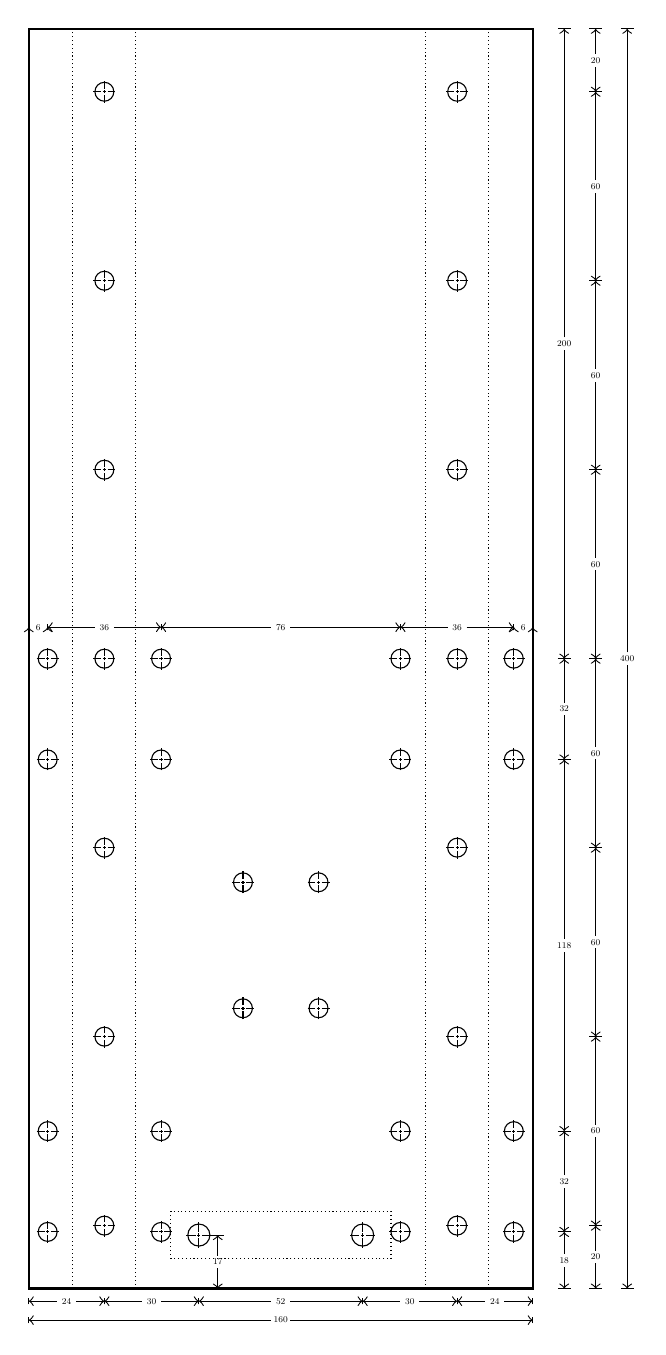
\begin{tikzpicture}[scale=0.4, every node/.style={scale=0.4}]
	% raw plate: 16cm x 40cm x 15mm
	% scale 2:5
	\draw[thick] (0, 0) rectangle (16, 40);
	\draw[densely dotted] (1.4, 0) -- (1.4, 40);
	\draw[densely dotted] (3.4, 0) -- (3.4, 40);
	\draw[densely dotted] (12.6, 0) -- (12.6, 40);
	\draw[densely dotted] (14.6, 0) -- (14.6, 40);
	
	\hole{2.4}{2}{3};
	\hole{2.4}{8}{3};
	\hole{2.4}{14}{3};
	\hole{2.4}{20}{3};
	\hole{2.4}{26}{3};
	\hole{2.4}{32}{3};
	\hole{2.4}{38}{3};
	\hole{13.6}{2}{3};
	\hole{13.6}{8}{3};
	\hole{13.6}{14}{3};
	\hole{13.6}{20}{3};
	\hole{13.6}{26}{3};
	\hole{13.6}{32}{3};
	\hole{13.6}{38}{3};
	
	% horizontal waggon mount - lower
	\hole{0.6}{1.8}{3};
	\hole{0.6}{5}{3};
	\hole{4.2}{1.8}{3};
	\hole{4.2}{5}{3};
	\hole{11.8}{1.8}{3};
	\hole{11.8}{5}{3};
	\hole{15.4}{1.8}{3};
	\hole{15.4}{5}{3};
	% horizontal waggon mount - upper
	\hole{0.6}{16.8}{3};
	\hole{0.6}{20}{3};
	\hole{4.2}{16.8}{3};
	\hole{4.2}{20}{3};
	\hole{11.8}{16.8}{3};
	\hole{11.8}{20}{3};
	\hole{15.4}{16.8}{3};
	\hole{15.4}{20}{3};
	% lower mount
	\hole{5.4}{1.7}{3.5};
	\hole{10.6}{1.7}{3.5};
	\draw[densely dotted] (4.5, 0.95) rectangle (11.5, 2.45);
	% horizontal spindle mount
	\hole{6.8}{8.9}{3};
	\hole{6.8}{12.9}{3};
	\hole{9.2}{8.9}{3};
	\hole{9.2}{12.9}{3};
	
	\dimsh{0}{2.4}{-0.4};
	\dimsh{2.4}{5.4}{-0.4};
	\dimsh{5.4}{10.6}{-0.4};
	\dimsh{10.6}{13.6}{-0.4};
	\dimsh{13.6}{16}{-0.4};
	\dimsh{0}{16}{-1};
	
	\dimsh{0}{0.6}{21};
	\dimsh{0.6}{4.2}{21};
	\dimsh{4.2}{11.8}{21};
	\dimsh{11.8}{15.4}{21};
	\dimsh{15.4}{16}{21};
	
	\dimsv{0}{1.8}{17};
	\dimsv{1.8}{5}{17};
	\dimsv{5}{16.8}{17};
	\dimsv{16.8}{20}{17};
	\dimsv{20}{40}{17};
	\dimsv{0}{2}{18};
	\dimsv{2}{8}{18};
	\dimsv{8}{14}{18};
	\dimsv{14}{20}{18};
	\dimsv{20}{26}{18};
	\dimsv{26}{32}{18};
	\dimsv{32}{38}{18};
	\dimsv{38}{40}{18};
	\dimsv{0}{40}{19};
	
	\dimsv{0}{1.7}{6};
	
	\end{tikzpicture}
	\caption{Spindle Z Mount - Main.}
	\label{fig:spindle_z_mount_main}
\end{figure}
\newpage
\begin{figure}[ht!]
	\centering
	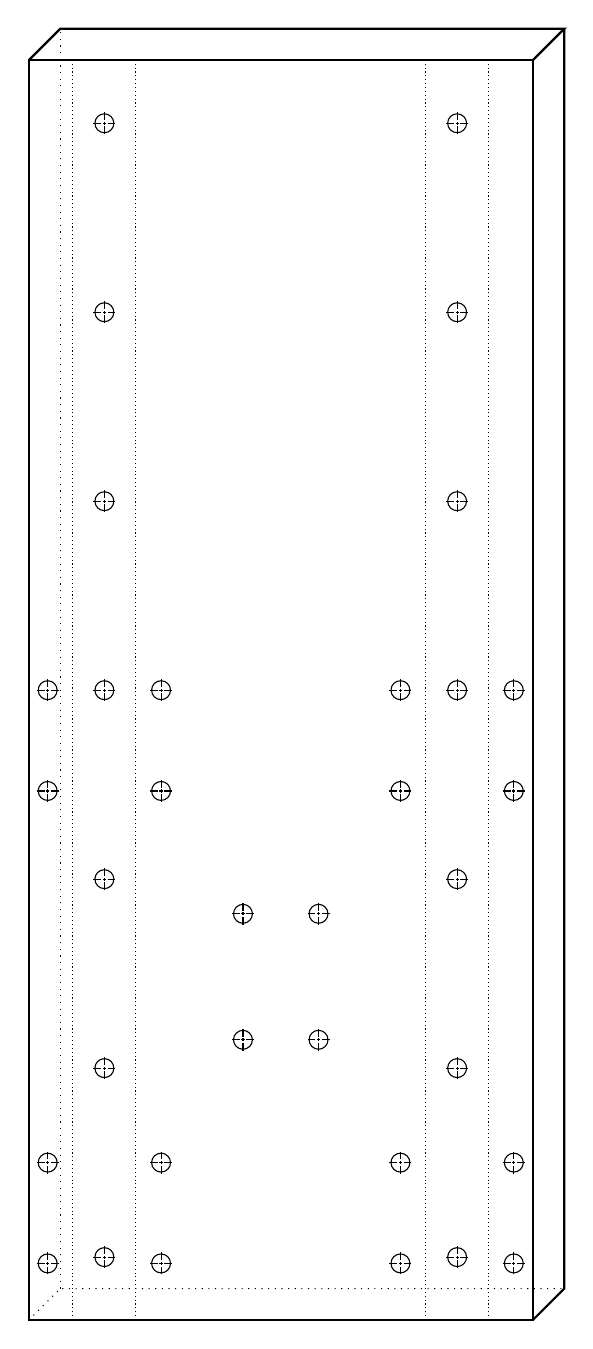
\begin{tikzpicture}[scale=0.4, every node/.style={scale=0.4}]
	% raw plate: 16cm x 40cm x 15mm
	% scale 2:5
	\draw[thick] (0, 0) rectangle (16, 40);
	\draw[thick] (0, 40) -- (1, 41) -- (17, 41) -- (16, 40);
	\draw[thick] (17, 41) -- (17, 1) -- (16, 0);
	\draw[dotted] (0, 0) -- (1, 1) -- (17, 1);
	\draw[dotted] (1, 1) -- (1, 41);
	\draw[densely dotted] (1.4, 0) -- (1.4, 40);
	\draw[densely dotted] (3.4, 0) -- (3.4, 40);
	\draw[densely dotted] (12.6, 0) -- (12.6, 40);
	\draw[densely dotted] (14.6, 0) -- (14.6, 40);
	
	\hole{2.4}{2}{3};
	\hole{2.4}{8}{3};
	\hole{2.4}{14}{3};
	\hole{2.4}{20}{3};
	\hole{2.4}{26}{3};
	\hole{2.4}{32}{3};
	\hole{2.4}{38}{3};
	\hole{13.6}{2}{3};
	\hole{13.6}{8}{3};
	\hole{13.6}{14}{3};
	\hole{13.6}{20}{3};
	\hole{13.6}{26}{3};
	\hole{13.6}{32}{3};
	\hole{13.6}{38}{3};
	
	% horizontal waggon mount - lower
	\hole{0.6}{1.8}{3};
	\hole{0.6}{5}{3};
	\hole{4.2}{1.8}{3};
	\hole{4.2}{5}{3};
	\hole{11.8}{1.8}{3};
	\hole{11.8}{5}{3};
	\hole{15.4}{1.8}{3};
	\hole{15.4}{5}{3};
	% horizontal waggon mount - upper
	\hole{0.6}{16.8}{3};
	\hole{0.6}{20}{3};
	\hole{4.2}{16.8}{3};
	\hole{4.2}{20}{3};
	\hole{11.8}{16.8}{3};
	\hole{11.8}{20}{3};
	\hole{15.4}{16.8}{3};
	\hole{15.4}{20}{3};
	% horizontal spindle mount
	\hole{6.8}{8.9}{3};
	\hole{6.8}{12.9}{3};
	\hole{9.2}{8.9}{3};
	\hole{9.2}{12.9}{3};
	\end{tikzpicture}
	\caption{Spindle Z Mount - Main 3D.}
	\label{fig:spindle_z_mount_main_3d}
\end{figure}
\newpage
\subsubsection{Upper}
\begin{figure}[ht!]
	\centering
	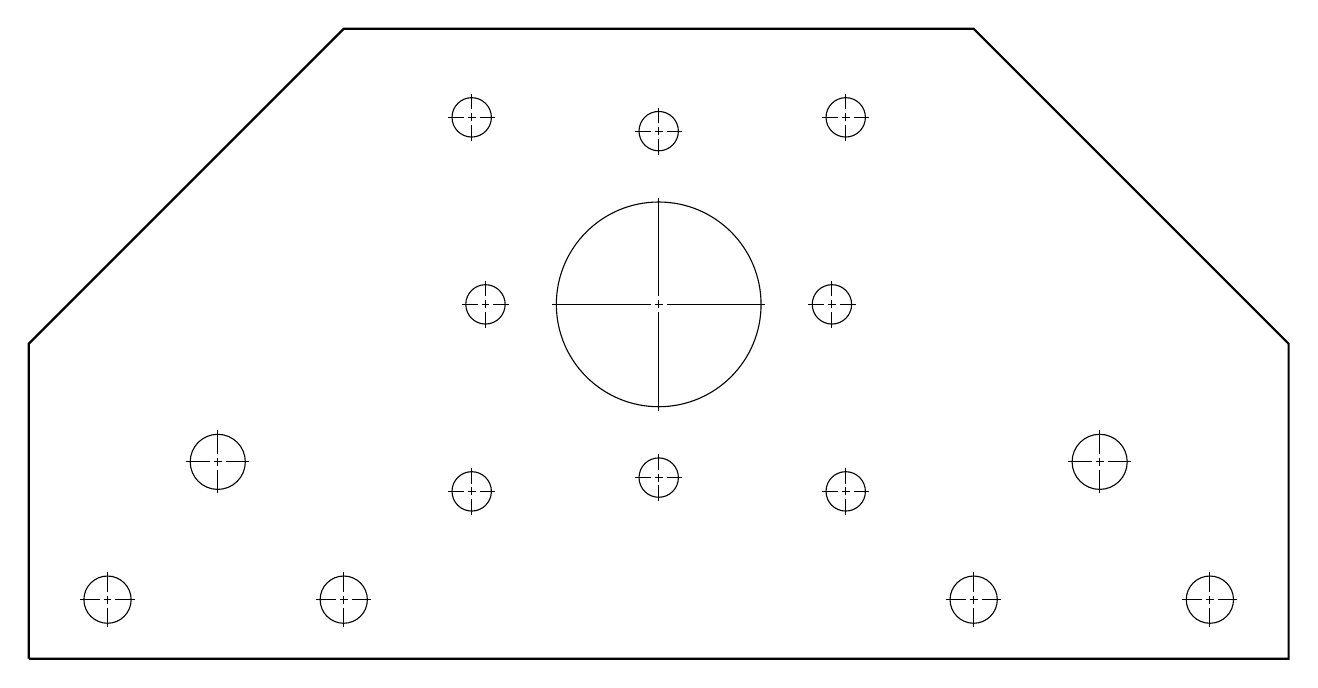
\begin{tikzpicture}
	% raw plate: 16cm x 8cm x 15mm
	% scale 1:1
	\draw[thick] (0, 0) -- (16, 0) -- (16, 4) -- (12, 8) -- (4, 8) -- (0, 4) -- (0, 0);
	
	\hole{1}{0.75}{3};
	\hole{4}{0.75}{3};
	\hole{12}{0.75}{3};
	\hole{15}{0.75}{3};
	
	\hole{2.4}{2.5}{3.5};
	\hole{13.6}{2.5}{3.5};
	
	\hole{8}{4.5}{13};
	
	\hole{5.8}{4.5}{2.5};
	\hole{8}{2.3}{2.5};
	\hole{8}{6.7}{2.5};
	\hole{10.2}{4.5}{2.5};
	
	\hole{5.625}{2.125}{2.5};
	\hole{5.625}{6.875}{2.5};
	\hole{10.375}{2.125}{2.5};
	\hole{10.375}{6.875}{2.5};
	\end{tikzpicture}
	\caption{Spindle Z Mount - Upper.}
	\label{fig:spindle_z_mount_upper}
\end{figure}
\newpage
\begin{figure}[ht!]
	\centering
	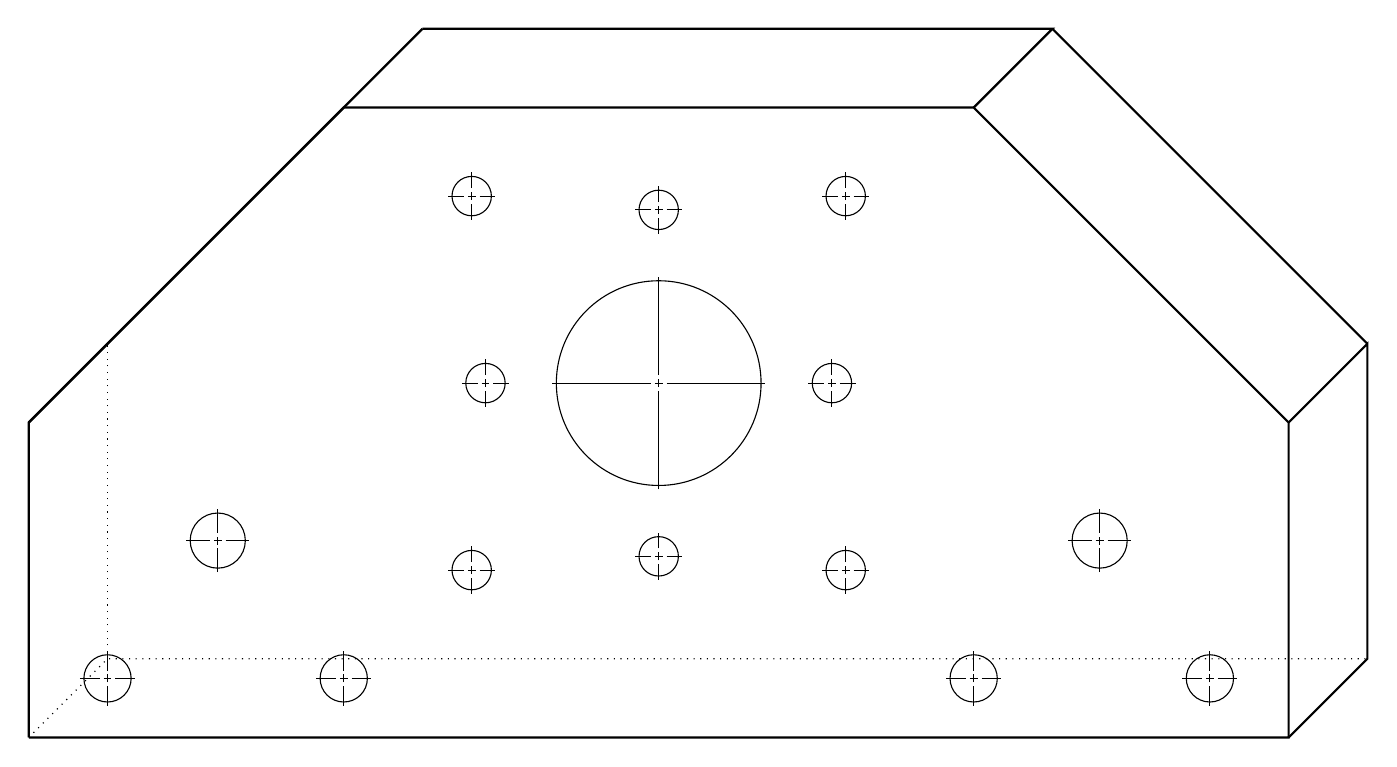
\begin{tikzpicture}
	% raw plate: 16cm x 8cm x 15mm
	% scale 1:1
	\draw[thick] (0, 0) -- (16, 0) -- (16, 4) -- (12, 8) -- (4, 8) -- (0, 4) -- (0, 0);
	\draw[thick] (0, 4) -- (1, 5) -- (5, 9) -- (4, 8);
	\draw[thick] (5, 9) -- (13, 9) -- (12, 8);
	\draw[thick] (13, 9) -- (17, 5);
	\draw[thick] (16, 4) -- (17, 5) -- (17, 1) -- (16, 0);
	\draw[dotted] (0, 0) -- (1, 1) -- (17, 1);
	\draw[dotted] (1, 1) -- (1, 5);
	\hole{1}{0.75}{3};
	\hole{4}{0.75}{3};
	\hole{12}{0.75}{3};
	\hole{15}{0.75}{3};
	
	\hole{2.4}{2.5}{3.5};
	\hole{13.6}{2.5}{3.5};
	
	\hole{8}{4.5}{13};
	
	\hole{5.8}{4.5}{2.5};
	\hole{8}{2.3}{2.5};
	\hole{8}{6.7}{2.5};
	\hole{10.2}{4.5}{2.5};
	
	\hole{5.625}{2.125}{2.5};
	\hole{5.625}{6.875}{2.5};
	\hole{10.375}{2.125}{2.5};
	\hole{10.375}{6.875}{2.5};
	\end{tikzpicture}
	\caption{Spindle Z Mount - Upper 3D.}
	\label{fig:spindle_z_mount_upper_3d}
\end{figure}
\newpage
\subsubsection{Lower}
Loslager FF12 will be connected to this part.
\begin{figure}[ht!]
	\centering
	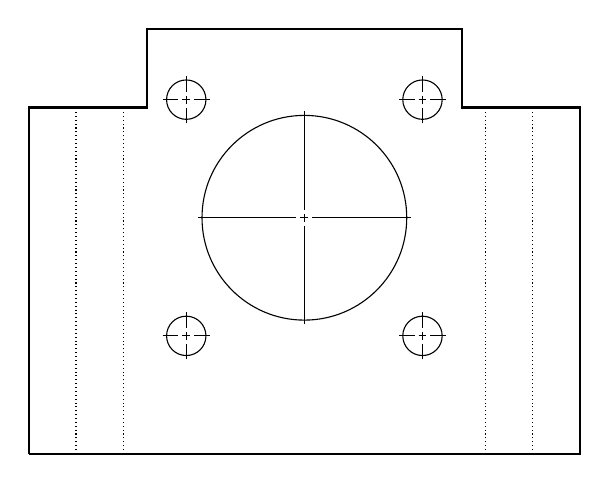
\begin{tikzpicture}
	% raw plate: 7cm x 5cm x 15mm
	% scale 1:1
	\draw[thick] (0, 0) -- (7, 0) -- (7, 4.4) -- (5.5, 4.4) -- (5.5, 5.4) -- (1.5, 5.4) -- (1.5, 4.4) -- (0, 4.4) -- (0, 0);
	\draw[densely dotted] (0.6, 0) --(0.6, 4.4);
	\draw[densely dotted] (1.2, 0) -- (1.2, 4.4);
	\draw[densely dotted] (5.8, 0) -- (5.8, 4.4);
	\draw[densely dotted] (6.4, 0) -- (6.4, 4.4);
	
	\hole{3.5}{3}{13};
	
	\hole{2}{1.5}{2.5};
	\hole{2}{4.5}{2.5};
	\hole{5}{1.5}{2.5};
	\hole{5}{4.5}{2.5};
	\end{tikzpicture}
	\caption{Spindle Z Mount - Lower.}
	\label{fig:spindle_z_mount_lower}
\end{figure}
\begin{figure}[ht!]
	\centering
	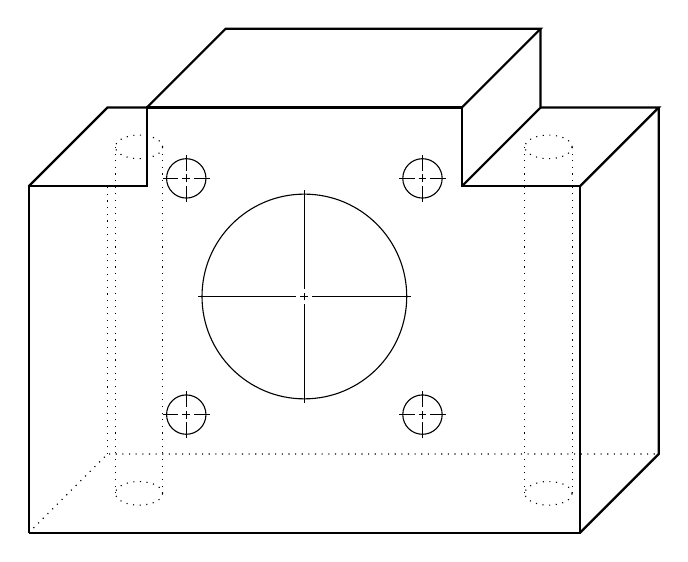
\begin{tikzpicture}
	% raw plate: 7cm x 5cm x 15mm
	% scale 1:1
	\draw[thick] (0, 0) -- (7, 0) -- (7, 4.4) -- (5.5, 4.4) -- (5.5, 5.4) -- (1.5, 5.4) -- (1.5, 4.4) -- (0, 4.4) -- (0, 0);
	\draw[thick] (0, 4.4) -- (1, 5.4) -- (1.5, 5.4);
	\draw[thick] (1.5, 5.4) -- (2.5, 6.4) -- (6.5, 6.4) -- (5.5, 5.4);
	\draw[thick] (6.5, 6.4) -- (6.5, 5.4) -- (5.5, 4.4);
	\draw[thick] (6.5, 5.4) -- (8, 5.4) -- (7, 4.4);
	\draw[thick] (8, 5.4) -- (8, 1) -- (7, 0);
	\draw[dotted] (0, 0) -- (1, 1) -- (8, 1);
	\draw[dotted] (1, 1) -- (1, 4.4);
	
	\draw[dotted] (1.4, 0.5) ellipse (3mm and 1.5mm);
	\draw[dotted] (1.4, 4.9) ellipse (3mm and 1.5mm);
	\draw[dotted] (1.1, 0.5) --(1.1, 4.9);
	\draw[dotted] (1.7, 0.5) -- (1.7, 4.9);
	\draw[dotted] (6.6, 0.5) ellipse (3mm and 1.5mm);
	\draw[dotted] (6.6, 4.9) ellipse (3mm and 1.5mm);
	\draw[dotted] (6.3, 0.5) -- (6.3, 4.9);
	\draw[dotted] (6.9, 0.5) -- (6.9, 4.9);
	
	\hole{3.5}{3}{13};
	
	\hole{2}{1.5}{2.5};
	\hole{2}{4.5}{2.5};
	\hole{5}{1.5}{2.5};
	\hole{5}{4.5}{2.5};
	\end{tikzpicture}
	\caption{Spindle Z Mount - Lower 3D.}
	\label{fig:spindle_z_mount_lower_3d}
\end{figure}
\newpage
\subsubsection{Drill Mount}
\begin{figure}[ht!]
	\centering
	\begin{tikzpicture}
	% raw plate: 16cm x 22cm x 15mm
	% scale 1:1
	\draw[thick] (3, 0) -- (13, 0) -- (13, 4) -- (16, 7) -- (16, 22) -- (0, 22) -- (0, 7) -- (3, 4) -- (3, 0);
	% drill mount
	\hole{4.5}{2}{3.5};
	\hole{4.5}{5.3}{3.5};
	\hole{11.5}{2}{3.5};
	\hole{11.5}{5.3}{3.5};
	% vertical waggon mount - lower
	\hole{0.8}{8}{3};
	\hole{0.8}{11.6}{3};
	\hole{4}{8}{3};
	\hole{4}{11.6}{3};
	\hole{12}{8}{3};
	\hole{12}{11.6}{3};
	\hole{15.2}{8}{3};
	\hole{15.2}{11.6}{3};
	% vertical waggon mount - upper
	\hole{0.8}{16.6}{3};
	\hole{0.8}{20.2}{3};
	\hole{4}{16.6}{3};
	\hole{4}{20.2}{3};
	\hole{12}{16.6}{3};
	\hole{12}{20.2}{3};
	\hole{15.2}{16.6}{3};
	\hole{15.2}{20.2}{3};
	% vertical spindle mount
	\hole{6}{12.9}{3};
	\hole{6}{15.3}{3};
	\hole{10}{12.9}{3};
	\hole{10}{15.3}{3};
	
	\end{tikzpicture}
	\caption{Drill Mount.}
	\label{fig:drill_mount}
\end{figure}
\newpage
\begin{figure}[ht!]
	\centering
	\begin{tikzpicture}
	% raw plate: 16cm x 22cm x 15mm
	% scale 1:1
	\draw[thick] (3, 0) -- (13, 0) -- (13, 4) -- (16, 7) -- (16, 22) -- (0, 22) -- (0, 7) -- (3, 4) -- (3, 0);
	\draw[thick] (0, 22) -- (1, 23) -- (17, 23) -- (16, 22);
	\draw[thick] (17, 23) -- (17, 8) -- (16, 7);
	\draw[thick] (17, 8) -- (14, 5) -- (13, 4);
	\draw[thick] (14, 5) -- (14, 1) -- (13, 0);
	\draw[dotted] (3, 0) -- (4, 1) -- (14, 1);
	\draw[dotted] (4, 1) -- (4, 5) -- (3, 4);
	\draw[dotted] (4, 5) -- (1, 8) -- (0, 7);
	\draw[dotted] (1, 8) -- (1, 23); 
	% drill mount
	\hole{4.5}{2}{3.5};
	\hole{4.5}{5.3}{3.5};
	\hole{11.5}{2}{3.5};
	\hole{11.5}{5.3}{3.5};
	% vertical waggon mount - lower
	\hole{0.8}{8}{3};
	\hole{0.8}{11.6}{3};
	\hole{4}{8}{3};
	\hole{4}{11.6}{3};
	\hole{12}{8}{3};
	\hole{12}{11.6}{3};
	\hole{15.2}{8}{3};
	\hole{15.2}{11.6}{3};
	% vertical waggon mount - upper
	\hole{0.8}{16.6}{3};
	\hole{0.8}{20.2}{3};
	\hole{4}{16.6}{3};
	\hole{4}{20.2}{3};
	\hole{12}{16.6}{3};
	\hole{12}{20.2}{3};
	\hole{15.2}{16.6}{3};
	\hole{15.2}{20.2}{3};
	% vertical spindle mount
	\hole{6}{12.9}{3};
	\hole{6}{15.3}{3};
	\hole{10}{12.9}{3};
	\hole{10}{15.3}{3};
	
	\end{tikzpicture}
	\caption{Drill Mount 3D.}
	\label{fig:drill_mount_3d}
\end{figure}
\newpage
\begin{figure}[ht!]
	\centering
	\begin{tikzpicture}
	% raw plate: 16cm x 13.8cm x 5mm
	% scale 1:1
	\draw[thick] (0, 0) rectangle (16, 13.8);
	% vertical waggon mount - lower
	\hole{0.8}{0.8}{3};
	\hole{0.8}{4.4}{3};
	\hole{4}{0.8}{3};
	\hole{4}{4.4}{3};
	\hole{12}{0.8}{3};
	\hole{12}{4.4}{3};
	\hole{15.2}{0.8}{3};
	\hole{15.2}{4.4}{3};
	% vertical waggon mount - upper
	\hole{0.8}{9.4}{3};
	\hole{0.8}{13}{3};
	\hole{4}{9.4}{3};
	\hole{4}{13}{3};
	\hole{12}{9.4}{3};
	\hole{12}{13}{3};
	\hole{15.2}{9.4}{3};
	\hole{15.2}{13}{3};
	% vertical spindle mount
	\hole{6}{5.7}{3};
	\hole{6}{8.1}{3};
	\hole{10}{5.7}{3};
	\hole{10}{8.1}{3};
	
	\end{tikzpicture}
	\caption{Drill Mount Support Plate.}
	\label{fig:drill_mount_support}
\end{figure}
\end{document}